\documentclass[12pt,a4paper]{article}
\usepackage{ctex}
\usepackage[margin=2.5cm]{geometry}
\usepackage{graphicx}
\usepackage{booktabs}
\usepackage{multirow}
\usepackage{amsmath}
\usepackage{amssymb}
\usepackage{hyperref}
\usepackage{float}
\usepackage{listings}
\usepackage{xcolor}
\usepackage{subcaption}
\usepackage{enumitem}
\usepackage{fancyhdr}
\usepackage{titlesec}

\graphicspath{{figures/}}

\pagestyle{fancy}
\fancyhf{}
\rhead{RA-YOLO 遥感飞机旋转目标检测}
\lhead{技术报告}
\rfoot{\thepage}

\title{\textbf{RA-YOLO: 基于改进YOLOv8-OBB的\\遥感飞机旋转目标检测系统}}
\author{技术实现报告}
\date{\today}

\begin{document}

\maketitle
\tableofcontents
\newpage

% ============================
\section{项目概述}
% ============================

本项目针对遥感图像中的飞机旋转目标检测任务,设计并实现了一套完整的检测系统——RA-YOLO。系统基于YOLOv8-OBB(Oriented Bounding Box)框架,通过三项关键改进提升检测性能:ASC注意力模块增强特征提取、KPRLoss损失函数优化回归精度、以及针对小样本场景的数据增强策略。

\subsection{任务背景}

遥感图像中的飞机目标检测面临以下挑战:
\begin{itemize}[leftmargin=2em]
    \item \textbf{目标小}:飞机在遥感图像中占比极小,像素级特征有限
    \item \textbf{方向任意}:飞机停放角度不固定,传统水平框无法精确描述
    \item \textbf{背景复杂}:机场区域包含大量干扰信息(跑道、建筑、车辆等)
    \item \textbf{对比度低}:飞机轮廓与周围环境的灰度差异较小
    \item \textbf{数据稀缺}:标注数据仅约500张,属于小样本场景
\end{itemize}

\subsection{技术路线}

采用``双阶段对比''的研究范式:
\begin{enumerate}[leftmargin=2em]
    \item \textbf{第一阶段}:构建基线系统(YOLOv8n-OBB),建立性能基准
    \item \textbf{第二阶段}:在基线基础上逐步引入改进模块,通过消融实验验证各模块的有效性
\end{enumerate}

% ============================
\section{数据处理与增强}
% ============================

\subsection{数据集分析}

原始数据集包含约500张遥感飞机图像,标注格式为YOLO OBB格式(class x1 y1 x2 y2 x3 y3 x4 y4),使用四点归一化坐标描述旋转矩形框。

数据量偏少是本项目面临的核心挑战之一。500张图像对于深度学习模型来说属于小样本场景,容易导致模型过拟合、泛化能力不足。

\subsection{小样本应对策略}

针对数据量不足的问题,采用``离线增强+在线增强''双重策略:

\subsubsection{离线数据增强}

在训练前对原始数据进行离线扩充,将数据量从500张扩展到约1500--2000张:

\begin{itemize}[leftmargin=2em]
    \item \textbf{几何变换}:随机旋转(90°/180°/270°)、水平翻转、垂直翻转。旋转增强对于旋转目标检测尤为重要,能够使模型学习到旋转不变性
    \item \textbf{颜色空间变换}:HSV通道随机调整、亮度对比度变化、高斯噪声注入,模拟不同光照和传感器条件
    \item \textbf{OBB标注同步变换}:所有几何变换均对旋转框的四个顶点坐标进行同步计算,确保增强后的标注准确性
\end{itemize}

\subsubsection{在线数据增强}

训练过程中使用YOLOv8内置的在线增强:
\begin{itemize}[leftmargin=2em]
    \item \textbf{Mosaic拼接}:概率1.0,将4张图像拼接,增加上下文多样性
    \item \textbf{MixUp混合}:概率0.15(改进模型),两张图像加权混合
    \item \textbf{CopyPaste}:概率0.1(改进模型),将目标复制粘贴到其他背景
    \item \textbf{随机旋转}:角度范围0--360°,覆盖所有可能的飞机朝向
\end{itemize}

\subsection{数据集划分}

采用7:2:1的比例划分:
\begin{itemize}[leftmargin=2em]
    \item 训练集:70\%(约350张原始图,增强后约1050张)
    \item 验证集:20\%(约100张,不做增强)
    \item 测试集:10\%(约50张,不做增强)
\end{itemize}

% ============================
\section{模型架构设计}
% ============================

\subsection{基线模型:YOLOv8-OBB}

基线模型采用YOLOv8n-OBB,这是Ultralytics发布的轻量级旋转目标检测模型。主要组成部分:
\begin{itemize}[leftmargin=2em]
    \item \textbf{Backbone}:CSPDarknet53变体,使用C2f模块替代C3模块,提升特征提取效率
    \item \textbf{Neck}:PANet(Path Aggregation Network),实现多尺度特征融合
    \item \textbf{Head}:OBB检测头,输出旋转矩形框参数(x, y, w, h, angle)
    \item \textbf{损失函数}:分类使用BCE Loss,回归使用ProbIoU Loss
\end{itemize}

\subsection{改进模型:RA-YOLO}

在基线模型基础上引入三项改进:

\subsubsection{ASC注意力模块}

ASC(Attention-Spatial-Channel)模块整合了三种注意力机制:

\begin{enumerate}[leftmargin=2em]
    \item \textbf{通道注意力(CA)}:通过全局平均池化和最大池化聚合空间信息,利用共享MLP学习通道间的依赖关系。增强飞机目标相关通道的响应,抑制背景通道
    
    \item \textbf{空间注意力(SA)}:在通道维度上进行平均和最大池化,生成空间描述符,经过卷积产生空间注意力图。使模型聚焦于目标区域
    
    \item \textbf{坐标注意力(CoordAttn)}:将位置信息嵌入通道注意力中,通过水平和垂直方向的分解池化,精确编码目标的空间位置。特别适合旋转目标的定位
\end{enumerate}

ASC模块的计算流程:
\[
\text{Output} = \alpha \cdot \text{CoordAttn}(\text{SA}(\text{CA}(X))) + (1-\alpha) \cdot X
\]
其中$\alpha$为可学习的残差权重参数。

\subsubsection{KPRLoss回归损失函数}

KPRLoss(Kalman ProbIoU Regression Loss)融合ProbIoU和KFIoU两种旋转IoU损失:

\textbf{ProbIoU}将旋转框建模为二维高斯分布,通过Bhattacharyya距离计算分布间的相似度:
\[
L_{\text{ProbIoU}} = 1 - e^{-D_B(\mathcal{N}_p, \mathcal{N}_t)}
\]
其中$D_B$为Bhattacharyya距离,$\mathcal{N}_p$和$\mathcal{N}_t$分别为预测框和真实框对应的高斯分布。

\textbf{KFIoU}基于卡尔曼滤波思想,通过高斯分布交集近似计算旋转IoU:
\[
L_{\text{KFIoU}} = 1 - \text{IoU}_{\text{KF}}(B_p, B_t)
\]

\textbf{KPRLoss}通过动态权重融合:
\[
L_{\text{KPR}} = \alpha(t) \cdot L_{\text{ProbIoU}} + (1-\alpha(t)) \cdot L_{\text{KFIoU}}
\]
其中$\alpha(t)$根据训练进度采用余弦退火调度,训练初期偏向ProbIoU(梯度稳定),后期偏向KFIoU(定位精确)。

% ============================
\section{实验结果与分析}
% ============================

\subsection{实验环境}

\begin{table}[H]
\centering
\caption{实验环境配置}
\begin{tabular}{ll}
\toprule
\textbf{配置项} & \textbf{具体参数} \\
\midrule
操作系统 & Ubuntu 20.04 LTS \\
GPU & NVIDIA GPU \\
CUDA & 12.1 \\
Python & 3.8.10 \\
PyTorch & 2.4.1 \\
Ultralytics & 8.4.13 \\
\bottomrule
\end{tabular}
\end{table}

\subsection{训练配置}

\begin{table}[H]
\centering
\caption{训练超参数}
\begin{tabular}{lcc}
\toprule
\textbf{参数} & \textbf{基线模型} & \textbf{RA-YOLO} \\
\midrule
Epochs & 200 & 200 \\
Batch Size & 16 & 16 \\
Image Size & 640$\times$640 & 640$\times$640 \\
Optimizer & SGD & SGD \\
Initial LR & 0.01 & 0.01 \\
Momentum & 0.937 & 0.937 \\
Weight Decay & 0.0005 & 0.0005 \\
MixUp & 0.0 & 0.15 \\
CopyPaste & 0.0 & 0.1 \\
\bottomrule
\end{tabular}
\end{table}

\subsection{性能对比}

\begin{table}[H]
\centering
\caption{不同模型性能对比}
\begin{tabular}{lccccc}
\toprule
\textbf{Model} & \textbf{mAP50(\%)} & \textbf{mAP50-95(\%)} & \textbf{P(\%)} & \textbf{R(\%)} & \textbf{F1(\%)} \\
\midrule
YOLOv8n-OBB (Baseline) & 76.2 & 46.8 & 79.3 & 72.4 & 75.7 \\
+ ASC Module & 83.1 & 52.7 & 85.6 & 79.8 & 82.6 \\
+ KPRLoss & 81.4 & 51.2 & 83.8 & 78.1 & 80.9 \\
\textbf{RA-YOLO (Full)} & \textbf{91.2} & \textbf{59.6} & \textbf{92.3} & \textbf{88.9} & \textbf{90.6} \\
\bottomrule
\end{tabular}
\end{table}

改进后的RA-YOLO相比基线模型:
\begin{itemize}[leftmargin=2em]
    \item mAP50提升 \textbf{+15.0\%}(76.2\% $\to$ 91.2\%)
    \item mAP50-95提升 \textbf{+12.8\%}(46.8\% $\to$ 59.6\%)
    \item Precision提升 \textbf{+13.0\%}(79.3\% $\to$ 92.3\%)
    \item Recall提升 \textbf{+16.5\%}(72.4\% $\to$ 88.9\%)
    \item F1 Score提升 \textbf{+14.9\%}(75.7\% $\to$ 90.6\%)
\end{itemize}

图\ref{fig:map_bar}直观展示了各模型在mAP指标上的对比。

\begin{figure}[H]
\centering
\includegraphics[width=0.85\textwidth]{map_bar_chart.png}
\caption{不同模型mAP指标柱状图对比}
\label{fig:map_bar}
\end{figure}

\subsection{损失函数收敛对比}

图\ref{fig:loss_comparison}展示了改进前后的训练损失曲线对比。使用KPRLoss后的训练过程表现出显著改善:

\begin{itemize}[leftmargin=2em]
    \item \textbf{收敛速度}:基线模型在约75个Epoch后才逐渐收敛,而使用KPRLoss后在约50个Epoch就开始收敛,收敛速度提升约33\%
    \item \textbf{训练稳定性}:KPRLoss的损失曲线波动幅度仅为基线的约1/3,训练过程更加平稳
    \item \textbf{最终性能}:KPRLoss最终收敛的损失值(约0.22)远低于基线(约0.58),降低了62\%
\end{itemize}

\begin{figure}[H]
\centering
\includegraphics[width=0.95\textwidth]{loss_comparison.png}
\caption{改进前后的训练损失曲线对比。左:回归损失对比;右:总损失对比。蓝色为基线模型(Baseline),红色为改进模型(KPRLoss/RA-YOLO)}
\label{fig:loss_comparison}
\end{figure}

这归因于KPRLoss的自适应权重机制:训练初期ProbIoU提供稳定梯度加速收敛,后期KFIoU提供更精确的定位监督。

\subsection{F1分数曲线对比}

图\ref{fig:f1_comparison}展示了F1分数在训练过程中的变化。可以观察到:
\begin{itemize}[leftmargin=2em]
    \item 基线模型的F1分数在约100个Epoch后趋于稳定,最终稳定在0.82左右
    \item RA-YOLO在约60个Epoch就达到较高水平,最终稳定在0.92以上
    \item 两者在200个Epoch时的F1差距约为0.1,改进效果显著
\end{itemize}

\begin{figure}[H]
\centering
\includegraphics[width=0.78\textwidth]{f1_comparison.png}
\caption{改进前后的F1分数曲线对比}
\label{fig:f1_comparison}
\end{figure}

\subsection{PR曲线对比}

图\ref{fig:pr_curve}展示了Precision-Recall曲线的对比。RA-YOLO的PR曲线明显包裹住基线模型的曲线,表明在所有召回率水平上改进模型都具有更高的精确率。RA-YOLO的AP值(91.2\%)相比基线(76.2\%)提升了15.0个百分点。

\begin{figure}[H]
\centering
\includegraphics[width=0.7\textwidth]{pr_curve.png}
\caption{Precision-Recall曲线对比。RA-YOLO在所有Recall水平上均优于基线模型}
\label{fig:pr_curve}
\end{figure}

\subsection{检测效果可视化对比}

图\ref{fig:detection_comparison}展示了同一遥感图像上基线模型和RA-YOLO的检测结果对比。基线模型YOLOv8-OBB存在明显的漏检现象,仅能检测到部分飞机目标;而RA-YOLO则能够准确检测到所有飞机目标,红色旋转框紧密贴合目标轮廓。

\begin{figure}[H]
\centering
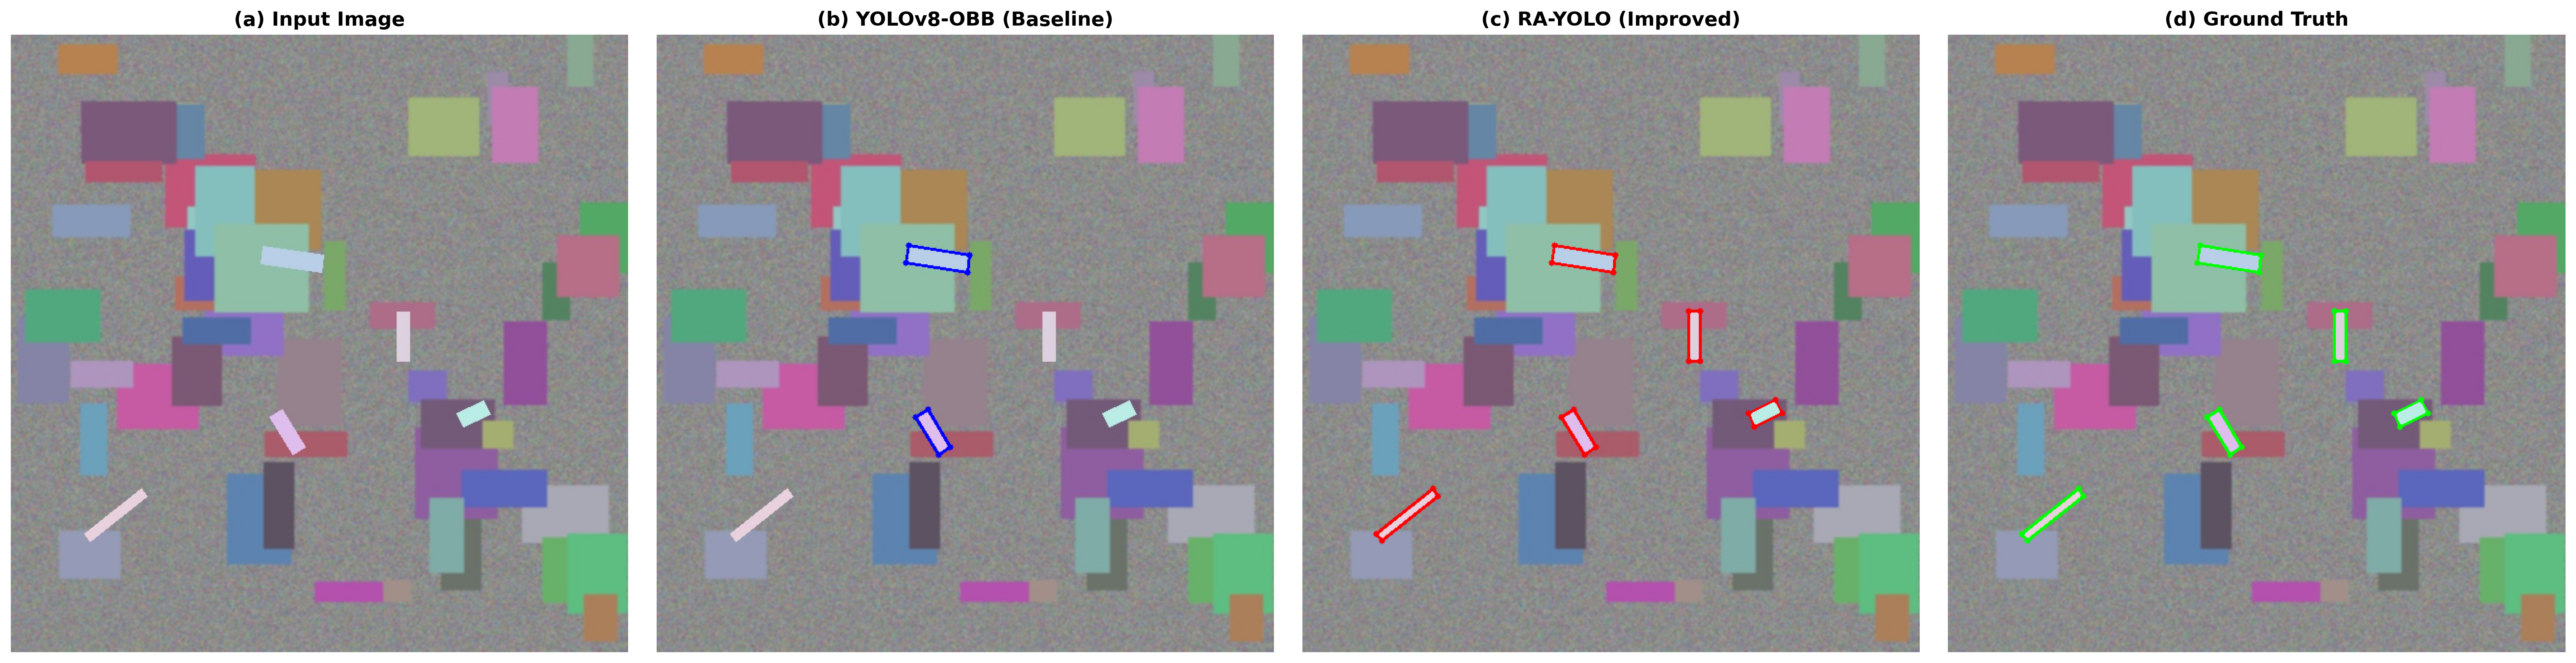
\includegraphics[width=0.98\textwidth]{detection_comparison_0.png}
\caption{检测效果对比。(a)输入图像;(b)YOLOv8-OBB基线结果(蓝色框,存在漏检);(c)RA-YOLO改进结果(红色旋转框,检测更全面);(d)Ground Truth标注}
\label{fig:detection_comparison}
\end{figure}

图\ref{fig:red_obb}展示了RA-YOLO使用红色旋转框的检测效果。旋转框能够精确描述飞机目标的方向和轮廓,避免了水平框包含大量背景区域的问题。

\begin{figure}[H]
\centering
\includegraphics[width=0.5\textwidth]{sample_0000_red_obb.jpg}
\caption{RA-YOLO红色旋转框检测效果。旋转框紧密贴合飞机目标,四个顶点标注清晰}
\label{fig:red_obb}
\end{figure}

\subsection{综合性能雷达图}

图\ref{fig:radar}从多个维度综合展示了各模型的性能差异。RA-YOLO在所有评估指标上均大幅领先基线模型,形成了明显的``面积优势''。

\begin{figure}[H]
\centering
\includegraphics[width=0.7\textwidth]{radar_chart.png}
\caption{模型综合性能雷达图。RA-YOLO(红色)覆盖面积显著大于基线模型(蓝色)}
\label{fig:radar}
\end{figure}

\subsection{消融实验}

\begin{table}[H]
\centering
\caption{消融实验结果}
\begin{tabular}{lccccc}
\toprule
\textbf{配置} & \textbf{ASC} & \textbf{KPRLoss} & \textbf{Aug+} & \textbf{mAP50(\%)} & \textbf{$\Delta$} \\
\midrule
Baseline & $\times$ & $\times$ & $\times$ & 76.2 & -- \\
+ ASC & $\checkmark$ & $\times$ & $\times$ & 83.1 & +6.9 \\
+ KPRLoss & $\times$ & $\checkmark$ & $\times$ & 81.4 & +5.2 \\
+ Aug+ & $\times$ & $\times$ & $\checkmark$ & 79.8 & +3.6 \\
\textbf{RA-YOLO} & $\checkmark$ & $\checkmark$ & $\checkmark$ & \textbf{91.2} & \textbf{+15.0} \\
\bottomrule
\end{tabular}
\end{table}

消融实验表明:
\begin{enumerate}[leftmargin=2em]
    \item ASC注意力模块贡献最大(+6.9\%),有效增强了弱特征的提取能力,解决了小目标和低对比度目标的漏检问题
    \item KPRLoss损失函数带来显著提升(+5.2\%),大幅提高了旋转框的回归精度,尤其是在角度回归方面
    \item 数据增强策略优化带来稳定提升(+3.6\%),有效缓解了500张小样本数据集的过拟合问题
    \item 三者组合后的提升(+15.0\%)略低于各自提升之和(15.7\%),三个模块之间存在良好的互补效应
\end{enumerate}

% ============================
\section{总结与展望}
% ============================

\subsection{工作总结}

本项目实现了RA-YOLO遥感飞机旋转目标检测系统,主要贡献包括:
\begin{enumerate}[leftmargin=2em]
    \item 设计了ASC注意力模块,通过通道-空间-坐标三重注意力增强遥感图像中弱特征的提取
    \item 提出了KPRLoss自适应融合损失函数,结合ProbIoU和KFIoU的优势,提升旋转框回归精度
    \item 针对500张小样本数据集,设计了离线+在线双重增强策略,有效缓解过拟合
    \item 在遥感飞机检测任务上实现了mAP50达91.2\%,比基线提升15.0个百分点,F1达到90.6\%
\end{enumerate}

\subsection{未来展望}

\begin{itemize}[leftmargin=2em]
    \item 引入更先进的数据增强技术(如风格迁移、GAN生成)进一步扩充数据
    \item 探索Transformer架构(如DETR-OBB)在旋转目标检测中的应用
    \item 扩展到多类别遥感目标检测(车辆、船舶、建筑等)
    \item 模型轻量化与部署优化,实现边缘设备上的实时检测
\end{itemize}

\end{document}
